\documentclass[border=4pt]{standalone}
\usepackage{tikz}
\usetikzlibrary{arrows.meta}
\definecolor{orangeText}{HTML}{E3A063}
\definecolor{orangeDim}{HTML}{A87A4E}
\begin{document}
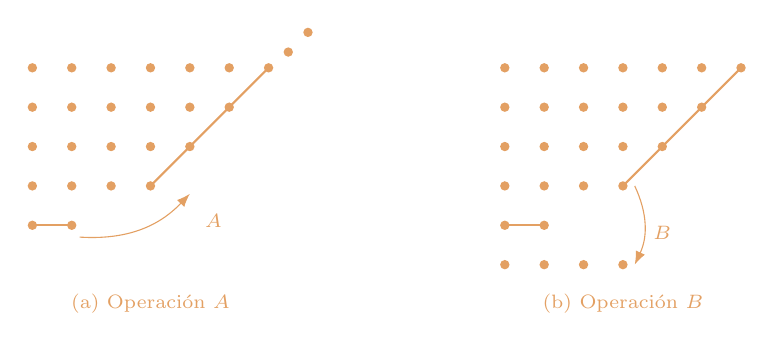
\begin{tikzpicture}[color=orangeText, scale=0.5,dot/.style={circle,fill,inner sep=1.2pt}]
  % (a) operation A
  \begin{scope}
    \foreach \len [count=\r from 0] in {7,6,5,4,2} {
      \foreach \c in {1,...,\len} \node[dot] at (\c,-\r) {};
    }
    \node[dot] at (8,0.9) {}; \node[dot] at (7.5,0.4) {};
    \draw[thick] (7,0) -- (4,-3);
    \draw[thick] (1,-4) -- (2,-4);
    \draw[-Latex] (2.2,-4.3) to[bend right=25] (5,-3.2);
    \node at (5.6,-3.9) {\scriptsize $A$};
    \node at (4,-6) {\scriptsize (a) Operación $A$};
  \end{scope}
  % (b) operation B
  \begin{scope}[xshift=12cm]
    \foreach \len [count=\r from 0] in {7,6,5,4,2} {
      \foreach \c in {1,...,\len} \node[dot] at (\c,-\r) {};
    }
    \foreach \c in {1,...,4} \node[dot] at (\c,-5) {};
    \draw[thick] (7,0) -- (4,-3);
    \draw[thick] (1,-4) -- (2,-4);
    \draw[-Latex] (4.3,-3) to[bend left=25] (4.3,-5);
    \node at (5,-4.2) {\scriptsize $B$};
    \node at (4,-6) {\scriptsize (b) Operación $B$};
  \end{scope}
\end{tikzpicture}
\end{document}
